\chapter{Algoritmi și Mecanici Principale}
\label{ch:algoritmi}

Complexitatea unui joc de strategie asimetric nu constă doar în logica vizuală sau în randarea graficii din client, ci și în eficiența sistemelor decizionale distribuite și în orchestrarea backend-ului. Acest capitol detaliază și analizează algoritmii centrali și arhitecturile concurente care guvernează funcționarea sistemului, accent-ul se pune pe eficiența computațională, gestionarea stărilor partajate și thread-safety.

\section{Algoritmul de Matchmaking și Gestiunea Instanțelor}
\label{sec:matchmaking}

Pentru a facilita conectarea jucătorilor într-un mediu competitiv multiplayer asimetric, a fost dezvoltat un serviciu de cuplare, ce a fost implementat pe serverul backend ASP.NET Core sub forma unui singleton coordonat asincron (\texttt{MatchmakingService}).

Acest sistem nu numai că asigură simpla asociere a doi utilizatori din coada de așteptare ci și acționează ca un orchestrator de procese Godot, fiind responsabil de crearea și izolarea instanțelor de execuție ale serverului de joc dedicat.

\subsection{Logica de Funcționare: Evaluare Imediată}
Algoritmul de matchmaking este proiectat după șablonul de arhitectură \textit{Producer-Consumer}, utilizând cozi de așteptare concurente, complet decuplate de firele de execuție care deservesc cererile HTTP/WebSocket ale clienților. Fluxul algoritmic este orchestrat de o clasă ce extinde \texttt{BackgroundService} din .NET, rulând o buclă infinită non-blocantă reglată prin semnale asincrone.

Etapele exacte ale algoritmului sunt descrise în continuare:
\begin{enumerate}
    \item \textbf{Înregistrarea Cererii (Production):} Jucătorul transmite o cerere de alocare specificând rolul dorit (\texttt{PlayerRole.Attacker} sau \texttt{PlayerRole.Defender}). Serverul validează jetonul de autentificare, generează un tichet unic de identificare și introduce referința utilizatorului în coada specifică rolului ales.
    \item \textbf{Evaluarea Concurentă (Consumption):} Bucla de fundal a serviciului interoghează starea cozilor dedicate. Evaluarea nu utilizează un mecanism primitiv de tip \textit{busy-waiting} (care ar epuiza resursele CPU), ci este trezită de mecanisme de sincronizare asincrone atunci când ambele cozi înregistrează elemente active. Când este îndeplinită condiția de existență a cel puțin unui candidat în fiecare structură (\texttt{AttackerQueue} și \texttt{DefenderQueue}), algoritmul extrage simultan cele două entități.
    \item \textbf{Alocarea Instanței și Pornirea Procesului Headless:} După extragerea cu succes, algoritmul generează un identificator unic global de meci (\texttt{MatchId} de tip GUID). Pentru a asigura o validare autoritară a meciului și a preveni trișarea (\textit{cheat prevention}), backend-ul nu deleagă logica către unul dintre clienți, ci instanțiază un proces separat, complet izolat, rulând executabilul Godot în mod \textit{Headless} (fără interfață grafică) pe sistemul de operare gazdă Linux/Ubuntu.

          Lansarea procesului se realizează programatic prin utilizarea clasei \texttt{System.Diagnostics.Process}, transmițând parametrii de configurare direct prin argumente în linie de comandă (CLI Args):
          \begin{itemize}
              \item Identificatorul unic al meciului (\texttt{--match-id});
              \item Configurația pachetelor de unități normalizate (\texttt{--defender-deck} și \texttt{--attacker-deck});
              \item Datele de profil sincronizate ale utilizatorilor (nume, indici de avatar).
          \end{itemize}
    \item \textbf{Persistența și Handshake-ul:} Starea meciului și configurarea inițială sunt persistate în baza de date relațională SQLite prin intermediul contextului Entity Framework Core. Clienții aflați în faza de așteptare recepționează asincron modificarea stării tichetului propriu și adresa instanței dedicate de Godot, inițiind faza de conexiune directă (Handshake) prin protocolul de rețea de nivel transport.
\end{enumerate}

% ---------------------------------------------------------
% PLACEHOLDER PENTRU DIAGRAMA FLOW MATCHMAKING
\begin{figure}[htbp]
    \centering
    % 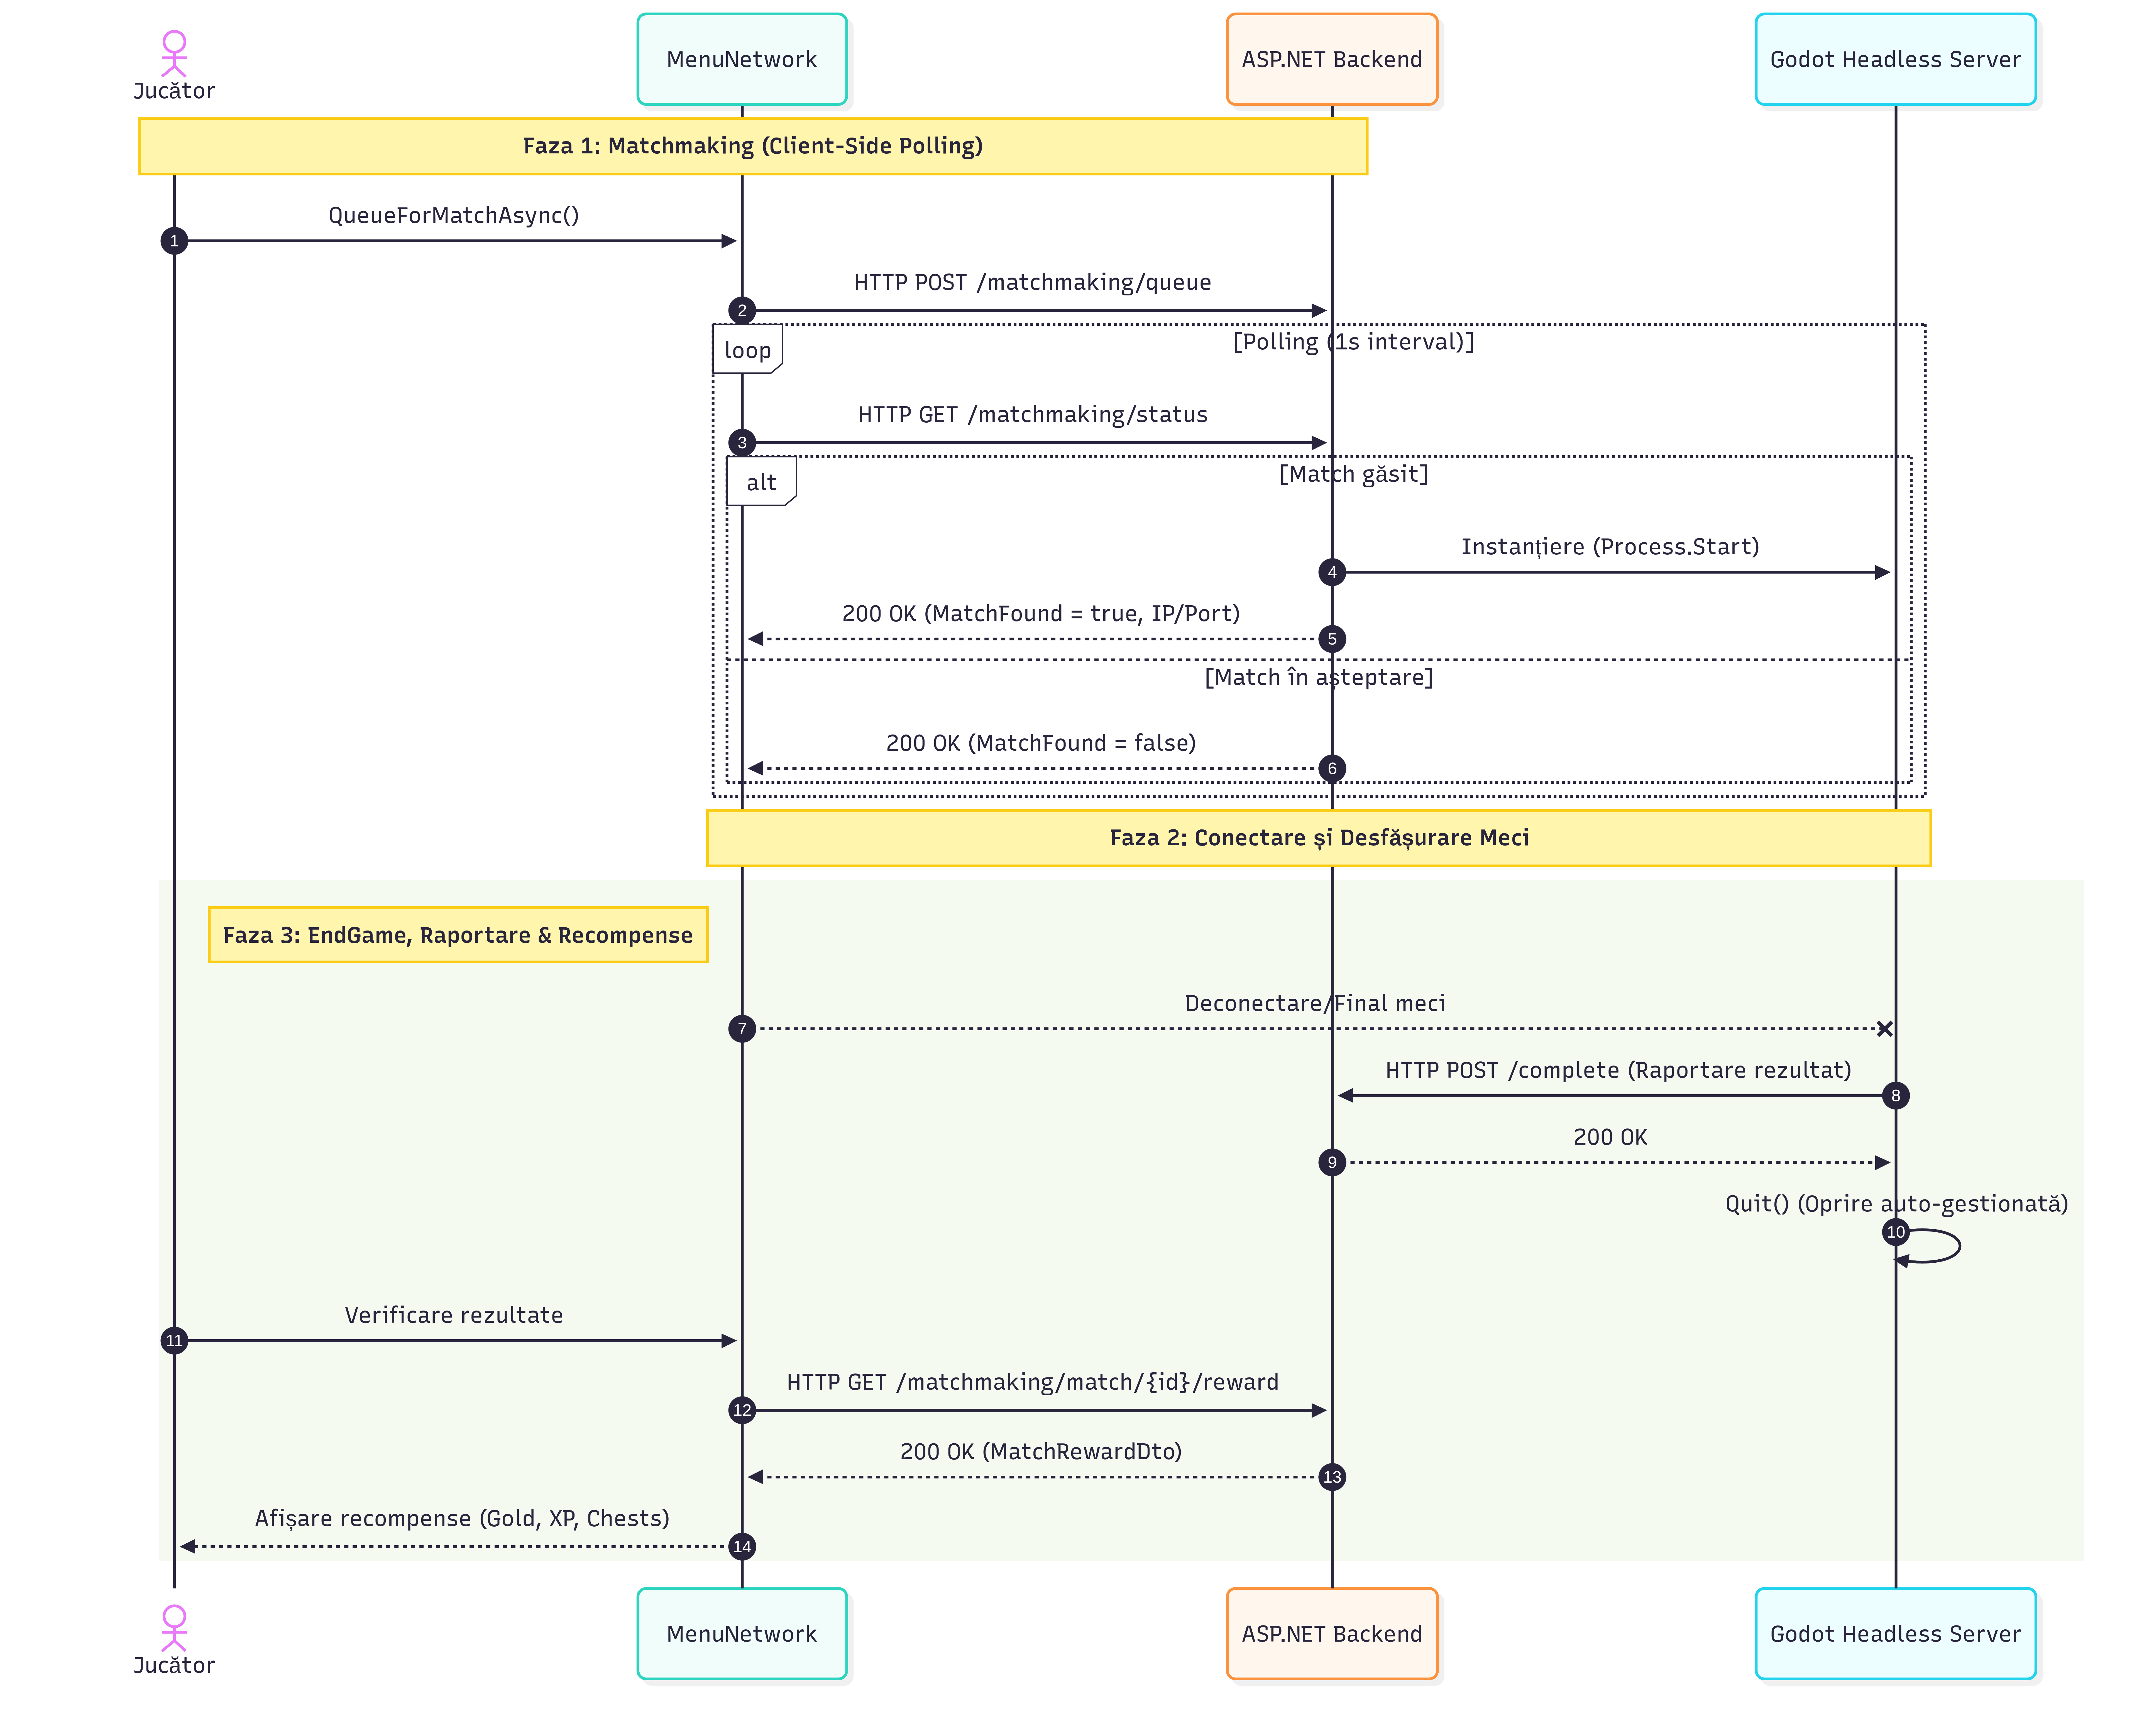
\includegraphics[width=\textwidth]{images/matchmaking-flow.png}
    \caption{Diagrama arhitecturală a sistemului de Matchmaking și ciclo-geneza serverului Headless}
    \label{fig:matchmaking_flow}
\end{figure}
% ---------------------------------------------------------

\subsection{Ciclul de Viață al Meciului și Toleranța la Eșec}
Odată instanțiat, serverul dedicat de Godot preia controlul absolut asupra simulării, funcționând după modelul \textit{Server-Authoritative}. Starea jocului (economia internă, timpul rămas și punctele de viață ale bazei) este calculată exclusiv pe server și propagată către clienți prin apeluri procedurale la distanță (RPC), prevenind astfel riscul de trișare prin manipularea memoriei locale a clientului.

Pentru a garanta robustețea sistemului în fața condițiilor reale de rețea, algoritmul de gestiune a meciului implementează multiple mecanisme de siguranță (Figura \ref{fig:matchmaking_flow}):
\begin{itemize}
    \item \textbf{Reziliența la Deconectări (Fault Tolerance):} În cazul pierderii conexiunii unui jucător, serverul nu oprește meciul imediat, ci inițiază o fereastră de grație asincronă (\texttt{Disconnect\-Grace\-Seconds}). Dacă utilizatorul nu reușește să restabilească o conexiune de nivel transport în intervalul de 30 de secunde, sistemul declară un abandon (\textit{forfeit}) în favoarea adversarului, asigurând fluiditatea experienței pentru jucătorii activi.
    \item \textbf{Comunicarea Inter-Procese (IPC):} La finalizarea condițiilor de victorie, instanța Headless comunică înapoi cu backend-ul ASP.NET Core printr-un apel HTTP autentificat. Raportarea rezultatului este validată folosind o cheie criptografică injectată în momentul ciclo-genezei (\texttt{MatchServerCallbackKey}), asigurând integritatea tranzacției de acordare a recompenselor (bani, experiență).
    \item \textbf{Prevenirea Proceselor Zombi:} În eventualitatea în care API-ul principal devine indisponibil și nu poate recepționa finalizarea meciului, instanța de joc folosește un \textit{safety timeout} local (\texttt{\_forceQuitTimer}). La expirarea acestuia, procesul de pe sistemul Linux se auto-termină forțat, prevenind astfel blocarea memoriei RAM (\textit{memory leaks}) și epuizarea resurselor infrastructurii (\textit{Resource Starvation}).
\end{itemize}

\subsection{Analiza Concurenței și Atomicitatea Tranzacțiilor}
Din punct de vedere computational, cozile de așteptare sunt implementate prin intermediul structurii de date \texttt{ConcurrentQueue<T>} furnizată de spațiul de nume \texttt{System.Collections.Concurrent}. Aceasta utilizează algoritmi lock-free bazați pe primitive atomice de tip \textit{Compare-And-Swap} (CAS), eliminând overhead-ul generat de blocajele tradiționale la nivel de kernel.

Operațiunile de adăugare (\texttt{Enqueue}) și extragere (\texttt{TryDequeue}) din cozile de așteptare se realizează în complexitate temporală constantă, amortizată $O(1)$. Prin urmare, algoritmul de împerechere prezintă o scalabilitate liniară în raport cu numărul de cereri concurente, limitarea fiind impusă exclusiv de resursele hardware (memorie și capacitate CPU pentru procesele Godot active în paralel).

Gestionarea concurenței este critică în momentul tranziției de la faza de cuplare la cea de instanțiere a procesului. Deoarece mai multe instanțe ale buclei asincrone sau cereri de anulare din partea utilizatorilor pot accesa simultan starea aceluiași tichet, operațiunile de scriere pe colecțiile de control ale stărilor active (\texttt{\_isProcessingRole}) sunt protejate prin secțiuni critice riguroase folosind mecanisme de excludere mutuală (\texttt{lock}).

Izolarea completă a logicii de simulare a jocului în procese \textit{Headless} distincte la nivelul nucleului Linux asigură că prăbușirea unei instanțe de joc din cauza unei erori de runtime nu afectează integritatea backend-ului ASP.NET Core sau a altor meciuri aflate în desfășurare, garantând o toleranță ridicată la eșec a întregului ecosistem.

\section{Sistemul Concurent de Sincronizare a Pachetului (Deck)}
\label{sec:deck_sync}

\subsection{Definirea Problemei și Abordarea Arhitecturală}
În aplicațiile interactive, manipularea rapidă a resurselor (ex. în proiectul curent: modificarea pachetelor de unități prin \textit{drag-and-drop}) implică apariția uonr provocări de sincronizare între client și server. Implementarea naivă ar fi recurgerea la apeluri HTTP sincrone, dar această abordare blochează interfața utilizatorului până la primirea răspunsului (Pessimistic Locking), ceea ce degradează semnificativ experiența vizuală.

Implementarea aleasă are în vedere principiul \textit{Server-Authoritative}, unde severul validează inputurile utilizatorului și deține informațiile finale despre starea jocului. Avantajele acestei abordări includ: fluiditatea interfeței, reducerea riscului de desincronizare și o experiență lipsită de sacadări vizuale.

\subsection{Coada Asincronă și Debouncing-ul Arhitectural}
Când utilizatorul solicită o mutare în pachetul de unități, componenta grafică deleagă noua configurație către serviciul (\texttt{DeckService}). Chiar dacă interfața vizuală rămâne interactivă și permite utilizatorului să efectueze noi mutări ale unităților (interacțiune non-blocantă), pachetul nu este actualizat instantaneu, ci așteaptă confirmarea serverului.

Pentru a preveni aglomerarea rețelei cu cereri HTTP la fiecare cadru (fenomen de \textit{spamming}) și a gestiona latența, serviciul implementează un mecanism de \textit{debouncing} cu excludere mutuală. Configurația solicitată este salvată într-un dicționar partajat (\texttt{\_pendingDeckByRole}), iar un identificator numeric de versiune (\texttt{\_latestVersionByRole}) este incrementat. Această operațiune este protejată de un blocaj \texttt{lock} (\textit{Thread Safety}).

O singură buclă asincronă (\texttt{ProcessSaveLoop}) este instanțiată pentru a iniția transmiterea datelor locale și a procesa modificările ce vin de pe server. Orice acțiune rapidă,  ulterioară a utilizatorului suprascrie pachetul ce este în așteptare pentru a fi actualizat pe server, fără a genera fire de execuție concurente.
% --- PLACEHOLDER DIAGRAMĂ DE SECVENȚĂ ---
\begin{figure}[htbp]
    \centering
    \includegraphics[width=0.85\textwidth]{images/async-debouncing-sync.png}
    \caption{Fluxul de sincronizare asincronă non-blocantă și anularea stărilor perimate}
    \label{fig:async_sync}
\end{figure}
% ----------------------------------------

\subsection{Validarea Răspunsurilor și Anularea Stărilor Precedente}
Deoarece cererile HTTP sunt procesate asincron, este prezent riscul ca răspunsurile de pe server să ajungă decalat (\textit{race conditions}). Sistemul rezolvă această problemă la finalizarea fiecărui apel (Figura \ref{fig:async_sync}).

Bucla evaluează dacă versiunea din momentul inițializării cererii coincide cu ultima versiune înregistrată la momentul primirii răspunsului (\texttt{IsLatestVersion}). Dacă utilizatorul a modificat pachetul de unități între timp, versiunea globală a fost deja actualizată(incrementată). În acest scenariu, răspunsul HTTP este considerat perimat (\textit{Stale Data}) și este ignorat, fără a declanșa vreo notificare pe ecran. Bucla extrage apoi noua configurație curentă a pachetului de unități și inițiază o nouă cerere către server.

Doar în momentul in care versiunile coincid, serviciul emite un semnal către clasa globală \texttt{GameState}, ce are ca scop actualizarea vizuală a interfeței grafice. Astfel, chiar dacă jucătorul a efectuat mutări/schimbări succesive rapide, UI-ul se va actualiza doar după rezultatul ultimei acțiuni, oferind o decuplare robustă și garantând că utilizatorul vede pe ecran numai starea confirmată de backend-ul \textit{ASP.NET Core}.